\documentclass[11pt, a4paper]{article}

% --- 基础宏包 ---
\usepackage[utf8]{inputenc}
\usepackage[T1]{fontenc}
\usepackage{xeCJK} % 中文支持
\usepackage{amsmath, amssymb} % 数学公式
\usepackage{geometry} % 页面布局
\usepackage{booktabs} % 规范表格
\usepackage{listings} % 代码块显示
\usepackage{xcolor} % 颜色设置
\usepackage{titlesec} % 标题格式定制
\usepackage{verbatim} % 保持原文格式(用于流程图)
\usepackage{graphicx} % 插入图片
\usepackage{indentfirst} % 每节首段也缩进

% --- 段落缩进设置 ---
\setlength{\parindent}{2em} % 首行缩进2个字符

% --- 页面边距设置 ---
\geometry{left=2.5cm, right=2.5cm, top=3cm, bottom=3cm}

% --- 代码块样式配置 ---
\lstset{
    language=Python,
    basicstyle=\ttfamily\small,
    keywordstyle=\color{blue},
    commentstyle=\color{gray},
    stringstyle=\color{orange},
    breaklines=true,
    frame=single,
    showstringspaces=false
} 

% --- 文档信息 ---
\title{\Huge \textbf{基于纯 Python 实现的 ResNet 图像分类器}}
\author{\Large 徐浩斌 \\ \large \texttt{kyochilian@gmail.com}}
\date{2026年1月2日}

\begin{document}

\maketitle
\tableofcontents
\newpage

\section{概述}
本项目旨在从零开始实现一个完整的深度卷积神经网络图像分类系统。标准如下:1、不依赖任何深度学习框架如 PyTorch 或 TensorFlow;2、不使用任何科学计算库如Numpy、Pandas,仅使用纯 Python 语言完成所有核心计算;3、手动推导所有反向传播公式并用python实现,使代码能够正常运行。

项目选择经典的残差网络 ResNet \cite{resnet} 作为主要架构,并在 MNIST 手写数字数据集 \cite{mnist} 上进行训练和评估。

现代深度学习框架虽然极大简化了模型开发流程,但其高度封装的特性也使得学习者难以真正理解前向传播与反向传播的具体计算过程。在学习过程中,尤其在数字图像处理这一门基础图像处理学科上,使用深度学习框架(例如直接使用torch.conv2d一类),
无论是Matlab还是python,都无法体现这门课的基础能力。通过手动实现每一层的前向计算和梯度反传,可以深刻体会到链式法则在神经网络中的应用 \cite{backprop},以及各种优化技巧背后的数学原理。
同时,也让我深刻体会到了,之前学习的并不是“深度学习”,而是“使用深度学习框架进行深度学习”。

真正重要的还是基础。

本项目实现的主要内容包括:基础矩阵运算库、全连接层、卷积层、批归一化层、激活函数、池化层、残差连接模块、SE 注意力模块、Bottleneck 结构等核心组件。同时还实现了交叉熵损失函数、SGD 优化器以及完整的训练流程。通过消融实验对比了不同网络结构的性能差异,验证了 BatchNorm \cite{batchnorm} 和残差连接对网络训练的重要作用。

\section{项目整体结构}
整个项目采用模块化设计,将不同功能划分到独立的文件中,便于维护和扩展。

\begin{figure}[htbp]
    \centering
    \includegraphics[width=0.4\textwidth,height=0.6\textwidth]{../pic/workspace.png} 
    \caption{项目整体架构图}
    \label{fig:workspace}
\end{figure}

核心文件包括矩阵运算模块 \texttt{matrix.py}、神经网络层模块 \texttt{layers.py}、ResNet 网络架构 \texttt{resnet.py}、消融实验模型 \texttt{ablation\_models.py}、损失函数 \texttt{loss.py}、优化器 \texttt{optimizer.py}、数据加载器 \texttt{dataloader.py} 以及训练脚本 \texttt{train.py} 和实验脚本 \texttt{run\_experiments.py}。

矩阵运算模块是整个项目的基础,它实现了一个自定义的 Matrix 类,支持多维数组的创建、索引、形状变换以及基本的数学运算。由于不使用 NumPy,所有的矩阵乘法、转置、求和等操作都通过嵌套的 Python 列表和循环来实现。

PS:在运行中,我发现,手写的速度远远低于Numpy科学计算库的速度,并且由于存在大量的浮点运算与矩阵运算,导致精度并不高。
但是,虽然这种方式在计算效率上远不如优化过的数值计算库,但在编写过程中清晰了这些运算的本质。

神经网络层模块是项目的核心部分,每一种网络层都继承自基类 Layer,并实现 forward 和 backward 两个关键方法。forward 方法负责前向传播的计算,同时将必要的中间结果缓存起来供反向传播使用。backward 方法根据上游传来的梯度,计算当前层参数的梯度以及需要继续向下游传播的输入梯度。这种统一的接口设计使得不同层可以像积木一样自由组合。

ResNet 网络架构模块定义了残差块 BasicBlock 和完整的 ResNet 模型 \cite{resnet}。残差块的核心思想是引入恒等映射的捷径连接,使得网络可以学习残差函数而非直接学习目标映射。这种设计有效缓解了深层网络的梯度消失问题。

消融实验模型模块包含了多种网络变体,用于验证各个组件的作用。其中 SimpleResNetNoBN 移除了所有的 BatchNorm 层,PlainNet 移除了残差连接,ResNetSE 则在 Bottleneck 结构基础上加入了 SE 通道注意力机制 \cite{senet}。通过对比这些变体的训练表现,可以直观地看到每个组件对网络性能的影响。

\subsection{本项目实现的 SimpleResNet 网络结构}
本项目实现的 SimpleResNet 是针对 MNIST \cite{mnist} 28×28 灰度图像设计的轻量级残差网络。完整的网络结构如下图所示,数据从输入层开始,依次经过初始卷积、两个残差块、全局平均池化,最后通过全连接层输出 10 个类别的预测概率:

\begin{figure}[htbp]
    \centering
    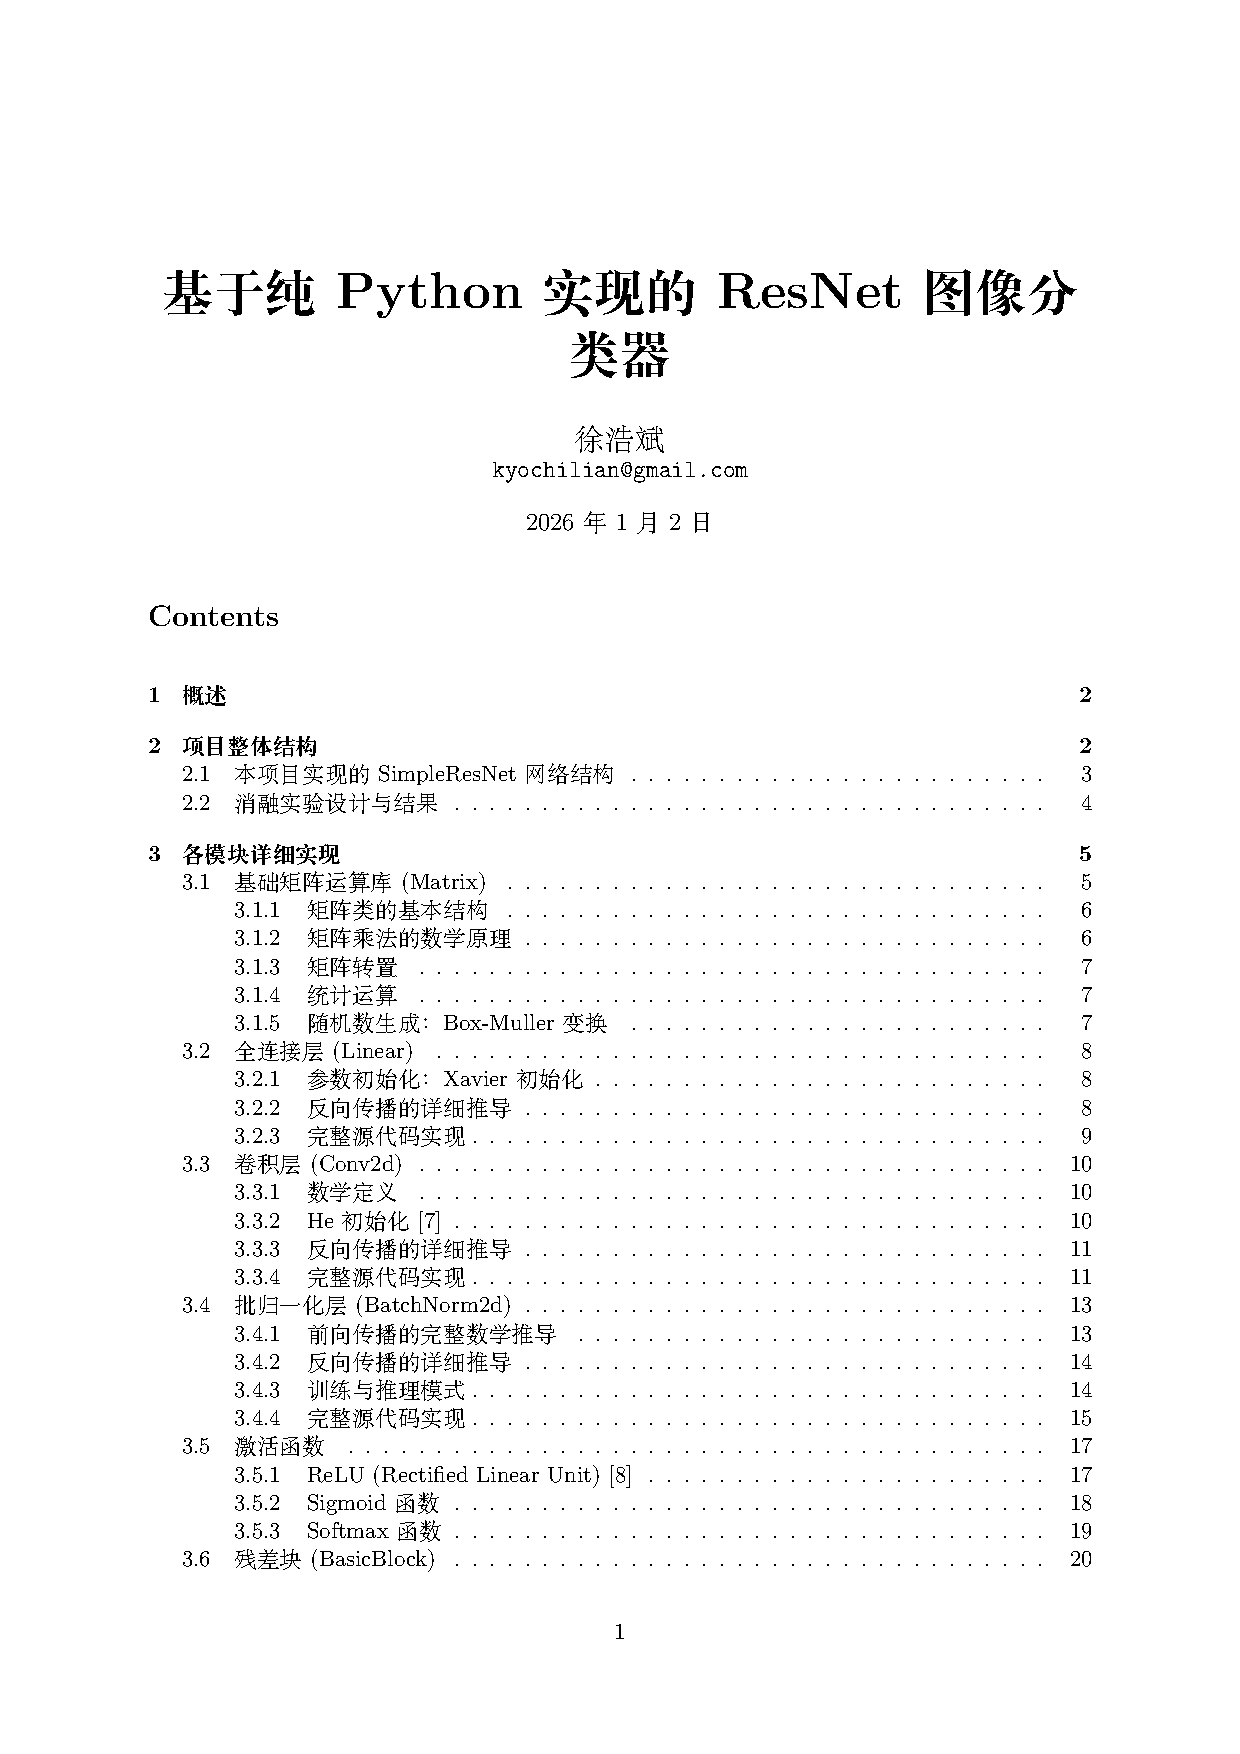
\includegraphics[width=0.8\textwidth]{../pic/resnet.jpg} 
    \caption{ResNet 网络结构图}
    \label{fig:resnet}
\end{figure}

网络设计遵循了 ResNet 的经典原则 \cite{resnet}:通道数逐渐增加的同时空间分辨率逐渐降低,最后通过全局平均池化消除空间维度。相比原始 ResNet-18 的上百层,这个简化版本仅包含 9 个卷积层,参数量约 5266 个,既保留了残差学习的核心思想,又能在纯 Python 环境下以可接受的速度运行。
但是这里的“可以接受”并不意味着在极大数据集与较多epoch和batch size下可以接受,下文会详细阐述,并说说我对于为什么要使用深度学习库的见解。

\subsection{消融实验设计与结果}
为验证各组件对网络性能的贡献,设计了四组对照实验。实验在 MNIST 数据集上进行,使用相同的训练配置(batch\_size=32, lr=0.005, epochs=10, 训练样本 5000)以保证公平比较。

注意:若采用完整的 ResNet-18 结构进行训练,模型参数量将达到数百万级别,在纯 Python 环境下训练时间将大幅增加,且可能面临内存不足的问题。因此,本项目的batch size和训练集、测试集的数量均大幅降低,以确保能够在合理时间内完成训练。
代价是:增建模块带来的效果不明显,且训练远远不如MLP稳定且高精度。毕竟,ResNet的优势在于其深层结构。

但是本项目的重点不在此,重要的是手写反向传播与各类模块的过程.如果愿意,可以让网络连续运行17小时(见图\ref{fig:完整运行网络的时间过长}),ResNet的精度一样可以达到99\%,证明模型本身和反向传播训练过程并没有任何问题。

\begin{table}[h!]
\centering
\begin{tabular}{@{}llllll@{}}
\toprule
模型名称 & 结构特点 & 参数量 & 最终训练准确率 & 最终测试准确率 & 平均 Epoch 时间 \\ \midrule
ResNet & 完整结构(残差+BN) & 5,266 & 40.2\% & 40.1\% & \textasciitilde{}275s \\
ResNetSE & 残差+BN+SE注意力 & 5,349 & 42.0\% & 41.1\% & \textasciitilde{}400s \\
NoBN & 移除所有 BatchNorm & 5,050 & 36.8\% & 39.0\% & \textasciitilde{}380s \\
PlainNet & 移除残差连接 & 5,266 & 30.1\% & 27.4\% & \textasciitilde{}275s \\ \bottomrule
\end{tabular}
\end{table}

\begin{figure}[htbp]
    \centering
    \includegraphics[width=0.9\textwidth]{../pic/ablation_study.png} 
    \caption{ResNet消融实验}
    \label{fig:ablation_study}
\end{figure}

\begin{figure}[htbp]
    \centering
    \includegraphics[width=0.8\textwidth]{../pic/training_curves.png} 
    \caption{运行曲线}
    \label{fig:training_curves}
\end{figure}

消融实验的结论是:BatchNorm 和残差连接都对网络的训练稳定性有重要贡献。移除 BatchNorm 后网络收敛变慢,训练初期准确率提升缓慢;移除残差连接后,深层梯度难以有效传播,整体性能下降。SE 注意力模块则通过学习通道间的依赖关系,有潜力进一步提升模型的表征能力,但也增加了计算开销。

可以看到,使用ResNet进行简单的训练的效果并不好。在笔者书写本报告时,有一个batch size=32,lr=0.001,epochs=20,训练集5000,测试集1000的网络正在运行,目前的精度已经到达了90\%以上。但它太慢,太慢,太慢了,并且经常运行到一半电脑就死机,推测是由于python长时间运行导致的内存泄漏问题。
\begin{figure}[htbp]
    \centering
    \includegraphics[width=0.8\textwidth]{../pic/full_run.png} 
    \caption{完整运行网络的时间过长}
    \label{fig:完整运行网络的时间过长}
\end{figure}

接下来是各个模块的原理以及核心实现,也是本报告的重中之重。


\section{各模块详细实现}

\subsection{基础矩阵运算库 (Matrix)}
本项目的核心基础是一个完全使用纯 Python 实现的矩阵运算库。该库不依赖 NumPy 等数值计算库,通过嵌套的 Python 列表存储多维数组数据,并实现了神经网络所需的全部数学运算。

并且,如果老师阅读到这一行,\textbf{我可以很明确地告诉您,我的所有公式、模块以及反向传播的推导过程,均由本人亲自完成,未借助任何辅助工具计算或者生成式人工智能。}
我学到了很多,并为此感到自豪。

\subsubsection{矩阵类的基本结构}
Matrix 类使用嵌套列表 \texttt{data} 存储数据,\texttt{shape} 元组记录各维度大小。支持 1D 到 4D 张量:

\begin{lstlisting}
class Matrix:
    def __init__(self, data):
        if isinstance(data, list):
            if len(data) == 0:
                self.data = []
                self.shape = (0,)
            elif isinstance(data[0], list):
                self.data = data
                self.shape = self._compute_shape(data)
            else:
                self.data = data
                self.shape = (len(data),)
        else:
            self.data = [[data]]
            self.shape = (1, 1)
    
    def _compute_shape(self, data):
        """递归计算数据的形状"""
        shape = []
        current = data
        while isinstance(current, list) and len(current) > 0:
            shape.append(len(current))
            current = current[0]
        return tuple(shape)
\end{lstlisting}

\subsubsection{矩阵乘法的数学原理}
给定矩阵 $\mathbf{A} \in \mathbb{R}^{m \times k}$ 和 $\mathbf{B} \in \mathbb{R}^{k \times n}$,矩阵乘法 $\mathbf{C} = \mathbf{A} \cdot \mathbf{B}$ 的定义为:
\begin{equation}\label{eq:resnet-auto-001}C_{ij} = \sum_{p=1}^{k} A_{ip} \cdot B_{pj}\end{equation}

这是一个三重循环的计算过程,时间复杂度为 $O(m \times k \times n)$(可以看出,时间复杂度非常高,这也是为什么自己手写计算的时间非常长):

\begin{lstlisting}
def matmul(self, other):
    """矩阵乘法 (2D @ 2D)"""
    if self.shape[1] != other.shape[0]:
        raise ValueError(f"Shape mismatch: {self.shape} @ {other.shape}")
    
    m, k = self.shape
    _, n = other.shape
    result = [[0.0 for _ in range(n)] for _ in range(m)]
    
    for i in range(m):
        for j in range(n):
            s = 0.0
            for p in range(k):
                s += self.data[i][p] * other.data[p][j]
            result[i][j] = s
    
    return Matrix(result)
\end{lstlisting}

\subsubsection{矩阵转置}
矩阵转置将行列互换:$(\mathbf{A}^T)_{ij} = A_{ji}$

\begin{lstlisting}
def T(self):
    """矩阵转置 (2D)"""
    if len(self.shape) == 2:
        rows, cols = self.shape
        result = [[self.data[i][j] for i in range(rows)] for j in range(cols)]
        return Matrix(result)
\end{lstlisting}

\subsubsection{统计运算}
这里的统计运算包括均值计算与方差计算,为后续的 BatchNorm 层提供支持:

均值计算:$\mu = \frac{1}{n}\sum_{i=1}^{n} x_i$

方差计算:$\sigma^2 = \frac{1}{n}\sum_{i=1}^{n} (x_i - \mu)^2$

\begin{lstlisting}
def mean(self, axis=None, keepdims=False):
    if axis is None:
        flat = self.flatten().data
        return sum(flat) / len(flat)
    # 支持多轴求平均,如 BatchNorm 需要在 (N, H, W) 上求平均

def var(self, axis=None, keepdims=False):
    if axis is None:
        flat = self.flatten().data
        m = sum(flat) / len(flat)
        return sum((x - m) ** 2 for x in flat) / len(flat)
\end{lstlisting}

\subsubsection{随机数生成:Box-Muller 变换}
神经网络的参数初始化需要正态分布随机数。Box-Muller 变换\cite{BoxMuller}是一种经典的随机数生成方法,由 George E. P. Box 和 Mervin E. Muller 于 1958 年提出。该方法能够将两个独立的均匀分布随机变量转换为两个独立的标准正态分布随机变量,在本网络实现中,用于生成符合 $\mathcal{N}(\text{mean}, \text{std}^2)$ 分布的随机数,用于后续的参数初始化。

给定两个独立的均匀分布随机变量 $U_1, U_2 \sim \text{Uniform}(0,1)$,可生成标准正态分布随机变量:
\begin{equation}\label{eq:resnet-auto-002}Z = \sqrt{-2\ln U_1} \cdot \cos(2\pi U_2)\end{equation}

\begin{lstlisting}
@staticmethod
def randn(shape, mean=0.0, std=1.0):
    """使用 Box-Muller 变换生成正态分布随机数"""
    def rand_normal():
        u1 = random.random()
        u2 = random.random()
        while u1 == 0:
            u1 = random.random()  # 避免 log(0)
        z = math.sqrt(-2.0 * math.log(u1)) * math.cos(2.0 * math.pi * u2)
        return mean + std * z
\end{lstlisting}

PS:1、这里的代码采用了递归的方式生成多维数组,递归的方法并不高效。在很多深度学习库的编写中,会尽量避免递归的出现,提升深度学习库的计算效率。

2、这里的随机数生成,我记得在python的基础库中存在,但我忘记了函数名称。或许并不存在能够生成正态分布随机变量的函数。不过自己写一遍总是好的。

\subsection{全连接层 (Linear)}
全连接层是最基础的神经网络层,每个输出神经元与所有输入神经元相连。

这也是本项目实现中第一个拦路虎。其实解决该模块的反向传播,该项目就已经完成了50\%,问题在于完成它。

\begin{figure}[htbp]
    \centering
    \includegraphics[width=0.8\textwidth]{../pic/linear.png} 
    \caption{全连接层示意}
    \label{fig:linear}
\end{figure}

给定输入向量 $\mathbf{x} \in \mathbb{R}^{d_{in}}$,权重矩阵 $\mathbf{W} \in \mathbb{R}^{d_{in} \times d_{out}}$ 和偏置向量 $\mathbf{b} \in \mathbb{R}^{d_{out}}$,前向传播的计算公式为:
\begin{equation}\label{eq:resnet-auto-003}\mathbf{y} = \mathbf{x} \cdot \mathbf{W} + \mathbf{b}\end{equation}

这也是老师上课时讲的,再熟悉不过的公式。
\subsubsection{参数初始化:Xavier 初始化}
为了保持前向传播时激活值的方差稳定,采用 Xavier 初始化\cite{xavier}:
\begin{equation}\label{eq:resnet-auto-004}\mathbf{W} \sim \mathcal{N}\left(0, \sqrt{\frac{2}{d_{in} + d_{out}}}\right)\end{equation}

这里的Xavier初始化是什么呢?简单来说,它是一种权重初始化方法,由 Glorot 和 Bengio 于 2010 年提出,旨在保持每层神经网络的输入和输出的方差相等,从而避免梯度消失或爆炸的问题。

Xavier初始化通过根据输入和输出神经元的数量来调整权重的初始分布,使得信号在网络中能够更稳定地传播。
\subsubsection{反向传播的详细推导}
设损失函数为 $L$,从上游传来的梯度为 $\frac{\partial L}{\partial \mathbf{y}}$(形状为 $(N, d_{out})$)。

\textbf{对权重的梯度:}

由于 $y_{nj} = \sum_{i} x_{ni} W_{ij} + b_j$,根据链式法则:
\begin{equation}\label{eq:resnet-auto-005}\frac{\partial L}{\partial W_{ij}} = \sum_{n} \frac{\partial L}{\partial y_{nj}} \cdot \frac{\partial y_{nj}}{\partial W_{ij}} = \sum_{n} \frac{\partial L}{\partial y_{nj}} \cdot x_{ni}\end{equation}

写成矩阵形式:
\begin{equation}\label{eq:resnet-auto-006}\frac{\partial L}{\partial \mathbf{W}} = \mathbf{x}^T \cdot \frac{\partial L}{\partial \mathbf{y}}\end{equation}

\textbf{对偏置的梯度:}

由于 $y_{nj} = \sum_{i} x_{ni} W_{ij} + b_j$,偏置 $b_j$ 对所有样本的 $y_{nj}$ 都有贡献:
\begin{equation}\label{eq:resnet-auto-007}\frac{\partial L}{\partial b_j} = \sum_{n} \frac{\partial L}{\partial y_{nj}} \cdot \frac{\partial y_{nj}}{\partial b_j} = \sum_{n} \frac{\partial L}{\partial y_{nj}}\end{equation}

\textbf{对输入的梯度(用于继续反向传播):}
\begin{equation}\label{eq:resnet-auto-008}\frac{\partial L}{\partial x_{ni}} = \sum_{j} \frac{\partial L}{\partial y_{nj}} \cdot \frac{\partial y_{nj}}{\partial x_{ni}} = \sum_{j} \frac{\partial L}{\partial y_{nj}} \cdot W_{ij}\end{equation}

写成矩阵形式:
\begin{equation}\label{eq:resnet-auto-009}\frac{\partial L}{\partial \mathbf{x}} = \frac{\partial L}{\partial \mathbf{y}} \cdot \mathbf{W}^T\end{equation}

可以看出,全连接层的反向传播主要依赖于矩阵乘法和求和操作,同时链式法则的推导是层层递进的。我们可以根据偏导进行计算各层的梯度。

\subsubsection{完整源代码实现}
\begin{lstlisting}
class Linear(Layer):
    """全连接层"""
    
    def __init__(self, in_features, out_features, bias=True):
        super().__init__()
        self.in_features = in_features
        self.out_features = out_features
        self.use_bias = bias
        
        # Xavier 初始化 \cite{xavier}
        std = math.sqrt(2.0 / (in_features + out_features))
        self.params['weight'] = randn((in_features, out_features), std=std)
        if bias:
            self.params['bias'] = zeros((out_features,))
    
    def forward(self, x):
        """
        x: (batch_size, in_features)
        输出: (batch_size, out_features)
        """
        self.cache['input'] = x
        
        # y = x @ W + b
        out = x @ self.params['weight']
        if self.use_bias:
            for i in range(out.shape[0]):
                for j in range(out.shape[1]):
                    out.data[i][j] += self.params['bias'].data[j]
        return out
    
    def backward(self, dout):
        """
        dout: (batch_size, out_features)
        返回 dx: (batch_size, in_features)
        """
        x = self.cache['input']
        if len(x.shape) == 1:
            x = x.reshape((1, -1))
        
        # dW = x.T @ dout
        self.grads['weight'] = x.T() @ dout
        
        # db = sum(dout, axis=0)
        if self.use_bias:
            self.grads['bias'] = dout.sum(axis=0, keepdims=False)
        
        # dx = dout @ W.T
        dx = dout @ self.params['weight'].T()
        return dx
\end{lstlisting}

\subsection{卷积层 (Conv2d)}
卷积层是卷积神经网络的核心组件 \cite{lenet},它通过滑动卷积核在输入特征图上进行局部运算,既能提取空间特征,又大大减少了参数数量。

\subsubsection{数学定义}
给定输入特征图 $\mathbf{X} \in \mathbb{R}^{N \times C_{in} \times H \times W}$ 和卷积核 $\mathbf{K} \in \mathbb{R}^{C_{out} \times C_{in} \times k_h \times k_w}$,
其中$N$ 为批量大小,$C_{in}$ 和 $C_{out}$ 分别为输入和输出通道数,$H$ 和 $W$ 为输入特征图的高度和宽度,$k_h$ 和 $k_w$ 为卷积核的高度和宽度。偏置向量为 $\mathbf{b} \in \mathbb{R}^{C_{out}}$。
卷积运算的定义为:
\begin{equation}\label{eq:resnet-auto-010}\mathbf{Y}[n, c_o, h, w] = \sum_{c_i=0}^{C_{in}-1} \sum_{i=0}^{k_h-1} \sum_{j=0}^{k_w-1} \mathbf{X}[n, c_i, h \cdot s + i, w \cdot s + j] \cdot \mathbf{K}[c_o, c_i, i, j] + b[c_o]\end{equation}

其中 $s$ 为步长 stride。输出特征图的空间尺寸计算公式:
\begin{equation}\label{eq:resnet-auto-011}H_{out} = \left\lfloor \frac{H_{in} + 2 \cdot p - k_h}{s} \right\rfloor + 1, \quad W_{out} = \left\lfloor \frac{W_{in} + 2 \cdot p - k_w}{s} \right\rfloor + 1\end{equation}

\subsubsection{He 初始化 \cite{he_init}}
对于使用 ReLU 激活函数的网络,采用 He 初始化:
\begin{equation}\label{eq:resnet-auto-012}\mathbf{K} \sim \mathcal{N}\left(0, \sqrt{\frac{2}{C_{in} \times k_h \times k_w}}\right)\end{equation}

这里的He初始化是一种权重初始化方法,专门针对使用 ReLU 激活函数的神经网络设计。He 初始化通过调整权重的初始分布,确保在前向传播过程中激活值的方差保持稳定,从而有效缓解了梯度消失或爆炸的问题。

\begin{figure}[htbp]
    \centering
    \includegraphics[width=0.8\textwidth]{../pic/初始化.png} 
    \caption{前文提到的He初始化与Xavier初始化}
    \label{fig:初始化}
\end{figure}
\subsubsection{反向传播的详细推导}
卷积层的反向传播需要计算三个梯度,无论是公式还是时间复杂度,都非常复杂。设损失函数为 $L$,从上游传来的梯度为 $\frac{\partial L}{\partial \mathbf{Y}}$(形状为 $(N, C_{out}, H_{out}, W_{out})$)。  

\textbf{1. 对卷积核的梯度 $\frac{\partial L}{\partial \mathbf{K}}$:}

对于每个卷积核元素 $K[c_o, c_i, i, j]$,它参与了输出 $Y[n, c_o, h, w]$ 的计算,其中输入位置为 $(h \cdot s + i, w \cdot s + j)$。根据链式法则:
\begin{equation}\label{eq:resnet-auto-013}\frac{\partial L}{\partial K[c_o, c_i, i, j]} = \sum_n \sum_h \sum_w \frac{\partial L}{\partial Y[n, c_o, h, w]} \cdot X_{pad}[n, c_i, h \cdot s + i, w \cdot s + j]\end{equation}

\textbf{2. 对偏置的梯度 $\frac{\partial L}{\partial b}$:}
\begin{equation}\label{eq:resnet-auto-014}\frac{\partial L}{\partial b[c_o]} = \sum_n \sum_h \sum_w \frac{\partial L}{\partial Y[n, c_o, h, w]}\end{equation}

\textbf{3. 对输入的梯度 $\frac{\partial L}{\partial \mathbf{X}}$(转置卷积):}

输入 $X[n, c_i, h_i, w_i]$ 会影响多个输出位置。设 $h_i = h_o \cdot s + k_i$ 且 $w_i = w_o \cdot s + k_j$,则:
\begin{equation}\label{eq:resnet-auto-015}\frac{\partial L}{\partial X[n, c_i, h_i, w_i]} = \sum_{c_o} \sum_{h_o, w_o} \frac{\partial L}{\partial Y[n, c_o, h_o, w_o]} \cdot K[c_o, c_i, k_i, k_j]\end{equation}

其中 $(h_o, w_o, k_i, k_j)$ 满足 $h_i = h_o \cdot s + k_i$ 且 $w_i = w_o \cdot s + k_j$。

总而言之,这一大串公式是什么意思呢?通俗来说,就是卷积层的反向传播过程需要计算三个梯度:卷积核的梯度、偏置的梯度以及输入的梯度。每个梯度的计算都涉及到对上游梯度的加权求和,权重由输入数据或卷积核决定。通过链式法则,将这些梯度一层一层嵌套,层层递进,最终实现整个网络的反向传播。

\subsubsection{完整源代码实现}
\begin{lstlisting}
class Conv2d(Layer):
    """2D 卷积层"""
    
    def __init__(self, in_channels, out_channels, kernel_size, stride=1, padding=0, bias=True):
        super().__init__()
        self.kernel_size = kernel_size if isinstance(kernel_size, tuple) else (kernel_size, kernel_size)
        self.stride = stride if isinstance(stride, tuple) else (stride, stride)
        self.padding = padding if isinstance(padding, tuple) else (padding, padding)
        
        # He 初始化
        fan_in = in_channels * self.kernel_size[0] * self.kernel_size[1]
        std = math.sqrt(2.0 / fan_in)
        self.params['weight'] = randn((out_channels, in_channels, 
                                       self.kernel_size[0], self.kernel_size[1]), std=std)
        if bias:
            self.params['bias'] = zeros((out_channels,))
    
    def forward(self, x):
        n, c_in, h_in, w_in = x.shape
        kh, kw = self.kernel_size
        sh, sw = self.stride
        ph, pw = self.padding
        
        h_out = (h_in + 2 * ph - kh) // sh + 1
        w_out = (w_in + 2 * pw - kw) // sw + 1
        
        x_padded = self._pad(x, ph, pw)
        self.cache['input'] = x
        self.cache['input_padded'] = x_padded
        
        out = [[[[0.0 for _ in range(w_out)] for _ in range(h_out)] 
               for _ in range(self.out_channels)] for _ in range(n)]
        
        for ni in range(n):
            for co in range(self.out_channels):
                for ho in range(h_out):
                    for wo in range(w_out):
                        val = 0.0
                        for ci in range(c_in):
                            for ki in range(kh):
                                for kj in range(kw):
                                    hi = ho * sh + ki
                                    wi = wo * sw + kj
                                    val += x_padded.data[ni][ci][hi][wi] * \
                                           self.params['weight'].data[co][ci][ki][kj]
                        if self.use_bias:
                            val += self.params['bias'].data[co]
                        out[ni][co][ho][wo] = val
        return Matrix(out)
    
    def backward(self, dout):
        x_padded = self.cache['input_padded']
        n, c_in, h_in, w_in = self.cache['input'].shape
        _, c_out, h_out, w_out = dout.shape
        kh, kw = self.kernel_size
        sh, sw = self.stride
        ph, pw = self.padding
        
        # 初始化梯度
        dw = [[[[0.0 for _ in range(kw)] for _ in range(kh)] 
              for _ in range(c_in)] for _ in range(c_out)]
        dx_padded = [[[[0.0 for _ in range(w_in + 2*pw)] for _ in range(h_in + 2*ph)] 
                     for _ in range(c_in)] for _ in range(n)]
        
        for ni in range(n):
            for co in range(c_out):
                for ho in range(h_out):
                    for wo in range(w_out):
                        d = dout.data[ni][co][ho][wo]
                        for ci in range(c_in):
                            for ki in range(kh):
                                for kj in range(kw):
                                    hi = ho * sh + ki
                                    wi = wo * sw + kj
                                    # dW: 上游梯度 * 输入
                                    dw[co][ci][ki][kj] += x_padded.data[ni][ci][hi][wi] * d
                                    # dx: 上游梯度 * 权重
                                    dx_padded[ni][ci][hi][wi] += \
                                        self.params['weight'].data[co][ci][ki][kj] * d
        
        self.grads['weight'] = Matrix(dw)
        # 移除 padding 后返回 dx
        return Matrix(dx)
\end{lstlisting}

我们可以很清楚地看到,为了实现基本功能,卷积核心部分的for循环整整嵌套了7层!这导致极高的时间复杂度与极低的计算效率。这也是为什么在实际应用中,深度学习库都会使用高度优化的数值计算库(如 NumPy、CuPy、TensorFlow、PyTorch 等)来实现卷积运算,以提升计算速度和效率。
\subsection{批归一化层 (BatchNorm2d)}
批归一化 \cite{batchnorm} 是深度学习中最重要的技术之一,它通过标准化每层的输入分布来加速训练并提高稳定性。

\subsubsection{前向传播的完整数学推导}
对于卷积网络中的四维输入张量 $\mathbf{X} \in \mathbb{R}^{N \times C \times H \times W}$,BatchNorm 对每个通道 $c$ 独立进行标准化。设 $m = N \times H \times W$ 为每个通道的元素总数。

\textbf{第一步:计算通道均值}
\begin{equation}\label{eq:resnet-auto-016}\mu_c = \frac{1}{m} \sum_{n=1}^{N} \sum_{h=1}^{H} \sum_{w=1}^{W} x_{n,c,h,w}\end{equation}

\textbf{第二步:计算通道方差}
\begin{equation}\label{eq:resnet-auto-017}\sigma_c^2 = \frac{1}{m} \sum_{n=1}^{N} \sum_{h=1}^{H} \sum_{w=1}^{W} (x_{n,c,h,w} - \mu_c)^2\end{equation}

\textbf{第三步:标准化}
\begin{equation}\label{eq:resnet-auto-018}\hat{x}_{n,c,h,w} = \frac{x_{n,c,h,w} - \mu_c}{\sqrt{\sigma_c^2 + \epsilon}}\end{equation}

\textbf{第四步:仿射变换(可学习参数)}
\begin{equation}\label{eq:resnet-auto-019}y_{n,c,h,w} = \gamma_c \cdot \hat{x}_{n,c,h,w} + \beta_c\end{equation}

其中 $\gamma_c$ 和 $\beta_c$ 是可学习的缩放和平移参数。通俗来讲是什么意思呢?BatchNorm的前向传播过程可以分为四个步骤:计算均值、计算方差、标准化输入以及应用可学习的缩放和平移。这一过程有助于稳定训练过程,提高模型性能。
这里的仿射变换是指通过线性变换(缩放和平移)来调整标准化后的数据分布,就是让数据更加切合,微调。
\subsubsection{反向传播的详细推导}
BatchNorm 的反向传播是本项目中最复杂的部分之一,推导他要了我半条命。

在此感谢https://zhuanlan.zhihu.com/p/45614576的详细教学,让我理解了BatchNorm的反向传播过程。

设 $\frac{\partial L}{\partial y}$ 为上游梯度。

\textbf{对 $\gamma$ 的梯度:}
\begin{equation}\label{eq:resnet-auto-020}\frac{\partial L}{\partial \gamma_c} = \sum_{n,h,w} \frac{\partial L}{\partial y_{n,c,h,w}} \cdot \hat{x}_{n,c,h,w}\end{equation}

\textbf{对 $\beta$ 的梯度:}
\begin{equation}\label{eq:resnet-auto-021}\frac{\partial L}{\partial \beta_c} = \sum_{n,h,w} \frac{\partial L}{\partial y_{n,c,h,w}}\end{equation}

\textbf{对输入的梯度(最复杂):}

首先定义中间变量 $\frac{\partial L}{\partial \hat{x}} = \frac{\partial L}{\partial y} \cdot \gamma$。

由于 $\hat{x}$ 同时依赖于 $x$、$\mu$($x$ 的均值)和 $\sigma$($x$ 的标准差),需要考虑三条路径:

\begin{equation}\label{eq:resnet-auto-022}\frac{\partial L}{\partial x} = \frac{\partial L}{\partial \hat{x}} \cdot \frac{\partial \hat{x}}{\partial x} + \frac{\partial L}{\partial \hat{x}} \cdot \frac{\partial \hat{x}}{\partial \mu} \cdot \frac{\partial \mu}{\partial x} + \frac{\partial L}{\partial \hat{x}} \cdot \frac{\partial \hat{x}}{\partial \sigma} \cdot \frac{\partial \sigma}{\partial x}\end{equation}

最终化简结果:
\begin{equation}\label{eq:resnet-auto-023}\frac{\partial L}{\partial x_{n,c,h,w}} = \frac{1}{m \cdot \sigma_c} \left( m \cdot \frac{\partial L}{\partial \hat{x}_{n,c,h,w}} - \sum_{i} \frac{\partial L}{\partial \hat{x}_i} - \hat{x}_{n,c,h,w} \cdot \sum_{i} \frac{\partial L}{\partial \hat{x}_i} \cdot \hat{x}_i \right)\end{equation}

然而这个公式还是难以理解。我们拆开来看:

1. 第一项 $\frac{1}{m \cdot \sigma_c} \cdot m \cdot \frac{\partial L}{\partial \hat{x}_{n,c,h,w}}$:这是直接从标准化后的输出传递回输入的梯度,经过缩放。

2. 第二项 $-\frac{1}{m \cdot \sigma_c} \cdot \sum_{i} \frac{\partial L}{\partial \hat{x}_i}$:这是由于均值 $\mu$ 依赖于所有输入 $x_i$,所以需要减去均值对输入的影响。

3. 第三项 $-\frac{1}{m \cdot \sigma_c} \cdot \hat{x}_{n,c,h,w} \cdot \sum_{i} \frac{\partial L}{\partial \hat{x}_i} \cdot \hat{x}_i$:这是由于标准差 $\sigma$ 依赖于所有输入 $x_i$,所以需要减去标准差对输入的影响。 

\subsubsection{训练与推理模式}
训练时使用当前批次的统计量,同时更新运行均值和方差(用于推理):
\begin{equation}\label{eq:resnet-auto-024}\mu_{running} = (1-\alpha) \cdot \mu_{running} + \alpha \cdot \mu_{batch}\end{equation}

这里的 $\mu_{running}$ 表示运行均值,$\mu_{batch}$ 表示当前批次的均值,$\alpha$ 是动量参数,控制更新速度。

推理时使用累积的运行统计量,不再计算批次统计。

\subsubsection{完整源代码实现}
\begin{lstlisting}
class BatchNorm2d(Layer):
    """2D 批归一化层"""
    
    def __init__(self, num_features, eps=1e-5, momentum=0.1):
        super().__init__()
        self.num_features = num_features
        self.eps = eps
        self.momentum = momentum
        
        # 可训练参数
        self.params['gamma'] = ones((num_features,))
        self.params['beta'] = zeros((num_features,))
        
        # 运行时统计量(用于推理)
        self.running_mean = zeros((num_features,))
        self.running_var = ones((num_features,))
    
    def forward(self, x):
        n, c, h, w = x.shape
        
        if self.training:
            # 计算批量统计量
            mean = x.mean(axis=(0, 2, 3), keepdims=False)
            var = x.var(axis=(0, 2, 3), keepdims=False)
            
            # 更新运行统计量
            for ci in range(c):
                self.running_mean.data[ci] = (1 - self.momentum) * self.running_mean.data[ci] + \
                                             self.momentum * mean.data[ci]
                self.running_var.data[ci] = (1 - self.momentum) * self.running_var.data[ci] + \
                                            self.momentum * var.data[ci]
        else:
            mean = self.running_mean
            var = self.running_var
        
        # 标准化
        std = [math.sqrt(var.data[ci] + self.eps) for ci in range(c)]
        x_hat = [[[[0.0 for _ in range(w)] for _ in range(h)] for _ in range(c)] for _ in range(n)]
        
        for ni in range(n):
            for ci in range(c):
                for hi in range(h):
                    for wi in range(w):
                        x_hat[ni][ci][hi][wi] = (x.data[ni][ci][hi][wi] - mean.data[ci]) / std[ci]
        
        self.cache['x'] = x
        self.cache['x_hat'] = Matrix(x_hat)
        self.cache['std'] = std
        
        # 缩放和平移: y = gamma * x_hat + beta
        out = [[[[x_hat[ni][ci][hi][wi] * self.params['gamma'].data[ci] + 
                  self.params['beta'].data[ci]
                  for wi in range(w)] for hi in range(h)] for ci in range(c)] for ni in range(n)]
        return Matrix(out)
    
    def backward(self, dout):
        x_hat = self.cache['x_hat']
        std = self.cache['std']
        n, c, h, w = self.cache['x'].shape
        m = n * h * w
        
        # 计算 dgamma 和 dbeta
        dgamma = [0.0 for _ in range(c)]
        dbeta = [0.0 for _ in range(c)]
        for ni in range(n):
            for ci in range(c):
                for hi in range(h):
                    for wi in range(w):
                        dgamma[ci] += dout.data[ni][ci][hi][wi] * x_hat.data[ni][ci][hi][wi]
                        dbeta[ci] += dout.data[ni][ci][hi][wi]
        
        self.grads['gamma'] = Matrix(dgamma)
        self.grads['beta'] = Matrix(dbeta)
        
        # 计算 dx
        dx = [[[[0.0 for _ in range(w)] for _ in range(h)] for _ in range(c)] for _ in range(n)]
        for ci in range(c):
            gamma_c = self.params['gamma'].data[ci]
            std_c = std[ci]
            
            # 计算中间量
            dout_gamma_sum = 0.0
            dout_gamma_xhat_sum = 0.0
            for ni in range(n):
                for hi in range(h):
                    for wi in range(w):
                        dout_gamma = dout.data[ni][ci][hi][wi] * gamma_c
                        dout_gamma_sum += dout_gamma
                        dout_gamma_xhat_sum += dout_gamma * x_hat.data[ni][ci][hi][wi]
            
            dout_gamma_mean = dout_gamma_sum / m
            dout_gamma_xhat_mean = dout_gamma_xhat_sum / m
            
            for ni in range(n):
                for hi in range(h):
                    for wi in range(w):
                        dout_gamma = dout.data[ni][ci][hi][wi] * gamma_c
                        dx[ni][ci][hi][wi] = (dout_gamma - dout_gamma_mean - 
                                              x_hat.data[ni][ci][hi][wi] * dout_gamma_xhat_mean) / std_c
        return Matrix(dx)
\end{lstlisting}

可以看出,BatchNorm 的反向传播实现非常复杂,涉及多个嵌套循环和中间变量的计算。其中时间复杂度最高的地方在于计算输入梯度 `dx` 的部分,整整嵌套了5层循环!

\subsection{激活函数}
\begin{figure}[htbp]
    \centering
    \includegraphics[width=0.8\textwidth]{../pic/activate_func.png} 
    \caption{各类激活函数示意图}
    \label{fig:activate_func}
\end{figure}
激活函数为神经网络引入非线性,使网络能够学习复杂的非线性映射。没有激活函数,多层神经网络等价于单层线性变换。

\subsubsection{ReLU (Rectified Linear Unit) \cite{relu}}
ReLU 是目前最常用的激活函数,由 Nair 和 Hinton 于 2010 年提出,并在 AlexNet \cite{alexnet} 中得到广泛应用。其数学定义为:
\begin{equation}\label{eq:resnet-auto-025}\text{ReLU}(x) = \max(0, x) = \begin{cases} x & \text{if } x > 0 \\ 0 & \text{if } x \leq 0 \end{cases}\end{equation}

\textbf{ReLU 的反向传播:}

ReLU 的导数非常简单:
\begin{equation}\label{eq:resnet-auto-026}\frac{\partial \text{ReLU}(x)}{\partial x} = \begin{cases} 1 & \text{if } x > 0 \\ 0 & \text{if } x \leq 0 \end{cases} = \mathbf{1}_{[x>0]}\end{equation}

根据链式法则,反向传播时:
\begin{equation}\label{eq:resnet-auto-027}\frac{\partial L}{\partial x} = \frac{\partial L}{\partial y} \cdot \frac{\partial y}{\partial x} = \frac{\partial L}{\partial y} \cdot \mathbf{1}_{[x>0]}\end{equation}

即:上游梯度在 $x > 0$ 的位置保持不变,在 $x \leq 0$ 的位置变为 0。

\textbf{ReLU 源代码实现:}
\begin{lstlisting}
class ReLU(Layer):
    """ReLU 激活函数"""
    
    def forward(self, x):
        self.cache['input'] = x
        
        def _relu(data):
            if isinstance(data, list):
                return [_relu(item) for item in data]
            else:
                return max(0.0, data)
        
        return Matrix(_relu(x.data))
    
    def backward(self, dout):
        x = self.cache['input']
        
        def _relu_grad(x_data, dout_data):
            if isinstance(x_data, list):
                return [_relu_grad(x_item, d_item) 
                       for x_item, d_item in zip(x_data, dout_data)]
            else:
                return dout_data if x_data > 0 else 0.0
        
        return Matrix(_relu_grad(x.data, dout.data))
\end{lstlisting}

\subsubsection{Sigmoid 函数}
Sigmoid 函数将任意实数映射到 $(0, 1)$ 区间,常用于二分类输出或门控机制(如 SE 注意力模块):
\begin{equation}\label{eq:resnet-auto-028}\sigma(x) = \frac{1}{1 + e^{-x}}\end{equation}

\textbf{Sigmoid 的反向传播:}

Sigmoid 有一个优雅的导数性质:
\begin{equation}\label{eq:resnet-auto-029}\frac{d\sigma}{dx} = \sigma(x) \cdot (1 - \sigma(x))\end{equation}

这个是什么意思呢?它表示 Sigmoid 函数的导数可以通过函数值本身来表示,这使得反向传播计算更加简洁高效。

推导过程:
\begin{equation}\label{eq:resnet-auto-030}\frac{d\sigma}{dx} = \frac{d}{dx}\left(\frac{1}{1+e^{-x}}\right) = \frac{e^{-x}}{(1+e^{-x})^2} = \frac{1}{1+e^{-x}} \cdot \frac{e^{-x}}{1+e^{-x}} = \sigma(x) \cdot (1-\sigma(x))\end{equation}

根据链式法则:
\begin{equation}\label{eq:resnet-auto-031}\frac{\partial L}{\partial x} = \frac{\partial L}{\partial y} \cdot \sigma(x) \cdot (1 - \sigma(x))\end{equation}

\textbf{注意}

当 $x$ 非常大或非常小时,指数运算可能溢出。实现中需要限制输入范围:

\textbf{Sigmoid 源代码实现:}
\begin{lstlisting}
class Sigmoid(Layer):
    """Sigmoid 激活函数,用于 SE 注意力模块"""
    
    def forward(self, x):
        self.cache['input'] = x
        
        def _sigmoid(data):
            if isinstance(data, list):
                return [_sigmoid(item) for item in data]
            else:
                # 数值稳定性:限制输入范围
                val = max(-500, min(500, data))
                return 1.0 / (1.0 + math.exp(-val))
        
        out = Matrix(_sigmoid(x.data))
        self.cache['output'] = out
        return out
    
    def backward(self, dout):
        """Sigmoid 反向传播: dx = dout * y * (1 - y)"""
        y = self.cache['output']
        
        def _sigmoid_grad(y_data, dout_data):
            if isinstance(y_data, list):
                return [_sigmoid_grad(yi, di) for yi, di in zip(y_data, dout_data)]
            else:
                return dout_data * y_data * (1 - y_data)
        
        return Matrix(_sigmoid_grad(y.data, dout.data))
\end{lstlisting}

\subsubsection{Softmax 函数}
Softmax函数在深度学习中的应用非常广泛,最广为人知的就是 Transformer \cite{transformer} 中的注意力机制。
\begin{figure}[htbp]
    \centering
    \includegraphics[width=0.6\textwidth]{../pic/softmax.png} 
    \caption{Softmax 函数示意图}
    \label{fig:softmax}
\end{figure}
Softmax 将 $C$ 个实数转换为概率分布,常用于多分类输出层:
\begin{equation}\label{eq:resnet-auto-032}\text{Softmax}(\mathbf{z})_i = \frac{e^{z_i}}{\sum_{j=1}^{C} e^{z_j}}\end{equation}

\textbf{注意}

为防止指数溢出,实际计算时减去最大值:
\begin{equation}\label{eq:resnet-auto-033}\text{Softmax}(\mathbf{z})_i = \frac{e^{z_i - \max(\mathbf{z})}}{\sum_{j=1}^{C} e^{z_j - \max(\mathbf{z})}}\end{equation}

\begin{lstlisting}
class Softmax(Layer):
    def forward(self, x):
        n, c = x.shape
        out = [[0.0 for _ in range(c)] for _ in range(n)]
        
        for ni in range(n):
            # 数值稳定性:减去最大值
            max_val = max(x.data[ni])
            exp_sum = 0.0
            exps = []
            for ci in range(c):
                e = math.exp(min(700, x.data[ni][ci] - max_val))
                exps.append(e)
                exp_sum += e
            for ci in range(c):
                out[ni][ci] = exps[ci] / exp_sum
        
        self.cache['output'] = Matrix(out)
        return Matrix(out)
\end{lstlisting}

\subsection{残差块 (BasicBlock)}
残差块是 ResNet \cite{resnet} 的核心创新。传统网络直接学习目标映射 $\mathcal{H}(\mathbf{x})$,而残差块学习残差映射 $\mathcal{F}(\mathbf{x}) = \mathcal{H}(\mathbf{x}) - \mathbf{x}$,最终输出为:
\begin{equation}\label{eq:resnet-auto-034}\mathbf{y} = \mathcal{F}(\mathbf{x}) + \mathbf{x}\end{equation}

\subsubsection{为什么残差学习有效}
在没有残差连接的情况下,深层网络需要直接拟合复杂的映射函数,这可能导致梯度消失或爆炸,训练困难。而引入残差连接后,深层的网络只需学习输入与输出之间的差异(残差),这通常是一个更简单的任务。同时,残差有效地保持了信息在深层网络中的传递,不至于信息丢失过于严重。

当输入输出维度不同(通道数变化或下采样)时,需要对捷径路径进行变换:
\begin{equation}\label{eq:resnet-auto-035}\mathbf{y} = \mathcal{F}(\mathbf{x}) + \mathbf{W}_s \mathbf{x}\end{equation}

其中 $\mathbf{W}_s$ 通常是 1×1 卷积实现的线性投影。

\subsubsection{反向传播的梯度分流}
设 $\mathbf{y} = \mathcal{F}(\mathbf{x}) + \mathbf{x}$,根据链式法则:
\begin{equation}\label{eq:resnet-auto-036}\frac{\partial L}{\partial \mathbf{x}} = \frac{\partial L}{\partial \mathbf{y}} \cdot \frac{\partial \mathbf{y}}{\partial \mathbf{x}} = \frac{\partial L}{\partial \mathbf{y}} \cdot \left( \frac{\partial \mathcal{F}}{\partial \mathbf{x}} + \mathbf{I} \right)\end{equation}

其中 $\mathbf{I}$ 是恒等矩阵。这意味着梯度可以通过两条路径流动:
\begin{itemize}
\item 主路径:$\frac{\partial L}{\partial \mathbf{y}} \cdot \frac{\partial \mathcal{F}}{\partial \mathbf{x}}$(通过卷积层)
\item 残差路径:$\frac{\partial L}{\partial \mathbf{y}} \cdot \mathbf{I}$(直接传递)
\end{itemize}

所以,在反向传播中,梯度是两部分梯度,也就是主路径和残差路径的和,虽然在代码实现中看起来像是两次加法操作,但实际上它们是梯度的分流与合流过程。

\subsubsection{完整源代码实现}
\begin{lstlisting}
class BasicBlock(Layer):
    """ResNet 基础残差块"""
    
    def __init__(self, in_channels, out_channels, stride=1):
        super().__init__()
        # 主路径: Conv -> BN -> ReLU -> Conv -> BN
        self.conv1 = Conv2d(in_channels, out_channels, 3, stride=stride, padding=1, bias=False)
        self.bn1 = BatchNorm2d(out_channels)
        self.relu1 = ReLU()
        self.conv2 = Conv2d(out_channels, out_channels, 3, stride=1, padding=1, bias=False)
        self.bn2 = BatchNorm2d(out_channels)
        
        # 捷径路径(维度变化时需要投影)
        self.use_shortcut_conv = (stride != 1) or (in_channels != out_channels)
        if self.use_shortcut_conv:
            self.shortcut_conv = Conv2d(in_channels, out_channels, 1, stride=stride, bias=False)
            self.shortcut_bn = BatchNorm2d(out_channels)
        
        self.relu2 = ReLU()
    
    def forward(self, x):
        self.cache['input'] = x
        
        # 主路径
        out = self.conv1.forward(x)
        out = self.bn1.forward(out)
        out = self.relu1.forward(out)
        out = self.conv2.forward(out)
        out = self.bn2.forward(out)
        
        # 捷径路径
        if self.use_shortcut_conv:
            shortcut = self.shortcut_conv.forward(x)
            shortcut = self.shortcut_bn.forward(shortcut)
        else:
            shortcut = x
        
        # 残差连接: y = F(x) + x
        out = self._add(out, shortcut)
        out = self.relu2.forward(out)
        return out
    
    def backward(self, dout):
        # ReLU2 反向
        dout = self.relu2.backward(dout)
        
        # 残差连接的梯度分流:加法的两个输入都获得相同的上游梯度
        d_main = dout      # 主路径梯度
        d_shortcut = dout  # 捷径路径梯度
        
        # 主路径反向: bn2 -> conv2 -> relu1 -> bn1 -> conv1
        d_main = self.bn2.backward(d_main)
        d_main = self.conv2.backward(d_main)
        d_main = self.relu1.backward(d_main)
        d_main = self.bn1.backward(d_main)
        d_main = self.conv1.backward(d_main)
        
        # 捷径路径反向
        if self.use_shortcut_conv:
            d_shortcut = self.shortcut_bn.backward(d_shortcut)
            d_shortcut = self.shortcut_conv.backward(d_shortcut)
        
        # 输入梯度 = 主路径梯度 + 捷径路径梯度
        dx = self._add(d_main, d_shortcut)
        return dx
\end{lstlisting}

\subsection{SE 注意力模块 (Squeeze-and-Excitation)}
SE 模块 \cite{senet} 是一种通道注意力机制,通过学习各通道的重要性权重来自适应地增强有用特征、抑制无用特征。

\begin{figure}[htbp]
    \centering
    \includegraphics[width=0.8\textwidth]{../pic/SE.png} 
    \caption{SE 注意力模块结构示意图}
    \label{fig:se_module}
\end{figure}

\subsubsection{前向传播的数学公式}
SE 模块包含三个步骤:

\textbf{第一步:Squeeze(全局平均池化)}

将空间维度压缩为单个统计量,获取每个通道的全局信息:
\begin{equation}\label{eq:resnet-auto-037}z_c = \frac{1}{H \times W} \sum_{h=1}^{H} \sum_{w=1}^{W} x_{c,h,w}\end{equation}

输出 $\mathbf{z} \in \mathbb{R}^C$ 是一个通道描述符。

\textbf{第二步:Excitation(门控机制)}

使用两个全连接层学习通道间的依赖关系:
\begin{equation}\label{eq:resnet-auto-038}\mathbf{s} = \sigma\left(\mathbf{W}_2 \cdot \text{ReLU}(\mathbf{W}_1 \cdot \mathbf{z})\right)\end{equation}

其中 $\mathbf{W}_1 \in \mathbb{R}^{C/r \times C}$ 和 $\mathbf{W}_2 \in \mathbb{R}^{C \times C/r}$,$r$ 是降维比例(reduction ratio),用于减少参数量。

\textbf{第三步:Scale(通道重标定)}

用学习到的权重对原始特征进行逐通道加权:
\begin{equation}\label{eq:resnet-auto-039}\tilde{x}_{c,h,w} = s_c \cdot x_{c,h,w}\end{equation}

\subsubsection{反向传播的详细推导}
SE 模块的反向传播需要处理多条梯度路径。这里的反向传播的思路,主要由作者放出的GitHub链接https://github.com/titu1994/keras-squeeze-excite-network提供。

设 $\mathbf{y} = \mathbf{s} \odot \mathbf{x}$(逐通道乘法),$\frac{\partial L}{\partial \mathbf{y}}$ 为上游梯度。

\textbf{对原始特征 $\mathbf{x}$ 的梯度(通过乘法):}
\begin{equation}\label{eq:resnet-auto-040}\frac{\partial L}{\partial x_{c,h,w}}\bigg|_{mul} = \frac{\partial L}{\partial y_{c,h,w}} \cdot s_c\end{equation}

\textbf{对缩放因子 $\mathbf{s}$ 的梯度:}
\begin{equation}\label{eq:resnet-auto-041}\frac{\partial L}{\partial s_c} = \sum_{h,w} \frac{\partial L}{\partial y_{c,h,w}} \cdot x_{c,h,w}\end{equation}

然后通过 Sigmoid、FC2、ReLU、FC1 反向传播得到 $\frac{\partial L}{\partial \mathbf{z}}$。

\textbf{通过 GlobalAvgPool 对 $\mathbf{x}$ 的梯度:}
\begin{equation}\label{eq:resnet-auto-042}\frac{\partial L}{\partial x_{c,h,w}}\bigg|_{gap} = \frac{1}{H \times W} \cdot \frac{\partial L}{\partial z_c}\end{equation}

\textbf{最终梯度(两条路径相加):}
\begin{equation}\label{eq:resnet-auto-043}\frac{\partial L}{\partial x_{c,h,w}} = \frac{\partial L}{\partial x_{c,h,w}}\bigg|_{mul} + \frac{\partial L}{\partial x_{c,h,w}}\bigg|_{gap}\end{equation}

\subsubsection{完整源代码实现}
\begin{lstlisting}
class SEBlock(Layer):
    """Squeeze-and-Excitation 注意力模块"""
    
    def __init__(self, channels, reduction=4):
        super().__init__()
        self.channels = channels
        
        # Squeeze: Global Average Pooling
        self.gap = GlobalAvgPool2d()
        
        # Excitation: FC -> ReLU -> FC -> Sigmoid
        reduced_channels = max(1, channels // reduction)
        self.fc1 = Linear(channels, reduced_channels)
        self.relu = ReLU()
        self.fc2 = Linear(reduced_channels, channels)
        self.sigmoid = Sigmoid()
    
    def forward(self, x):
        n, c, h, w = x.shape
        self.cache['input'] = x
        
        # Squeeze: (N, C, H, W) -> (N, C)
        squeezed = self.gap.forward(x)
        
        # Excitation: (N, C) -> (N, C)
        excited = self.fc1.forward(squeezed)
        excited = self.relu.forward(excited)
        excited = self.fc2.forward(excited)
        scale = self.sigmoid.forward(excited)
        
        self.cache['scale'] = scale
        
        # Scale: 广播乘法 (N, C) * (N, C, H, W) -> (N, C, H, W)
        out = [[[[x.data[ni][ci][hi][wi] * scale.data[ni][ci]
                  for wi in range(w)] for hi in range(h)]
                for ci in range(c)] for ni in range(n)]
        return Matrix(out)
    
    def backward(self, dout):
        x = self.cache['input']
        scale = self.cache['scale']
        n, c, h, w = x.shape
        
        # 1. 乘法反向传播
        d_scale = [[0.0 for _ in range(c)] for _ in range(n)]
        d_x_mul = [[[[0.0 for _ in range(w)] for _ in range(h)]
                   for _ in range(c)] for _ in range(n)]
        
        for ni in range(n):
            for ci in range(c):
                for hi in range(h):
                    for wi in range(w):
                        d_scale[ni][ci] += dout.data[ni][ci][hi][wi] * x.data[ni][ci][hi][wi]
                        d_x_mul[ni][ci][hi][wi] = dout.data[ni][ci][hi][wi] * scale.data[ni][ci]
        
        # 2-5. Sigmoid -> FC2 -> ReLU -> FC1 反向
        d_scale = Matrix(d_scale)
        d_fc2_out = self.sigmoid.backward(d_scale)
        d_relu_out = self.fc2.backward(d_fc2_out)
        d_fc1_out = self.relu.backward(d_relu_out)
        d_squeezed = self.fc1.backward(d_fc1_out)
        
        # 6. GlobalAvgPool 反向
        d_x_gap = self.gap.backward(d_squeezed)
        
        # 7. 合并两条路径的梯度
        dx = [[[[d_x_mul[ni][ci][hi][wi] + d_x_gap.data[ni][ci][hi][wi]
                 for wi in range(w)] for hi in range(h)]
               for ci in range(c)] for ni in range(n)]
        return Matrix(dx)
\end{lstlisting}

\subsection{Bottleneck 结构}
Bottleneck 是 ResNet-50/101/152 使用的更深的残差块结构,采用瓶颈设计来减少计算量。

\subsubsection{Bottleneck 的数学结构}
\begin{equation}\label{eq:resnet-auto-044}\mathbf{y} = \underbrace{\text{Conv}_{1\times1} \rightarrow \text{BN} \rightarrow \text{ReLU} \rightarrow \text{Conv}_{3\times3} \rightarrow \text{BN} \rightarrow \text{ReLU} \rightarrow \text{Conv}_{1\times1} \rightarrow \text{BN}}_{\mathcal{F}(\mathbf{x})} + \mathbf{x}\end{equation}

三层卷积的作用:
\begin{itemize}
\item 第一个 1×1 卷积:降维,减少通道数
\item 3×3 卷积:在低维空间进行空间卷积(计算量更小)
\item 第二个 1×1 卷积:升维,恢复通道数
\end{itemize}

\subsubsection{反向传播}
Bottleneck 的反向传播需要通过三个卷积层和三个 BN 层,但原理与 BasicBlock 相同:主路径和捷径路径的梯度最终相加。

\begin{lstlisting}
class Bottleneck(Layer):
    def __init__(self, in_channels, mid_channels, out_channels, stride=1):
        super().__init__()
        # 1x1 降维
        self.conv1 = Conv2d(in_channels, mid_channels, 1, stride=1, padding=0, bias=False)
        self.bn1 = BatchNorm2d(mid_channels)
        self.relu1 = ReLU()
        # 3x3 卷积
        self.conv2 = Conv2d(mid_channels, mid_channels, 3, stride=stride, padding=1, bias=False)
        self.bn2 = BatchNorm2d(mid_channels)
        self.relu2 = ReLU()
        # 1x1 升维
        self.conv3 = Conv2d(mid_channels, out_channels, 1, stride=1, padding=0, bias=False)
        self.bn3 = BatchNorm2d(out_channels)
        
    def backward(self, dout):
        dout = self.relu3.backward(dout)
        d_main = dout
        d_shortcut = dout
        
        # 主路径反向: bn3 -> conv3 -> relu2 -> bn2 -> conv2 -> relu1 -> bn1 -> conv1
        d_main = self.bn3.backward(d_main)
        d_main = self.conv3.backward(d_main)
        d_main = self.relu2.backward(d_main)
        d_main = self.bn2.backward(d_main)
        d_main = self.conv2.backward(d_main)
        d_main = self.relu1.backward(d_main)
        d_main = self.bn1.backward(d_main)
        d_main = self.conv1.backward(d_main)
        
        if self.use_shortcut_conv:
            d_shortcut = self.shortcut_bn.backward(d_shortcut)
            d_shortcut = self.shortcut_conv.backward(d_shortcut)
        
        dx = self._add(d_main, d_shortcut)
        return dx
\end{lstlisting}

\section{整体反向传播公式及实现细节}

\subsection{损失函数:交叉熵损失 (CrossEntropyLoss)}
交叉熵损失是多分类任务的标准损失函数 \cite{deeplearning, crossentropy},它实际上是 Softmax 和负对数似然的组合。

\subsubsection{Softmax 函数}
对原始 logits $\mathbf{z} \in \mathbb{R}^C$ 应用 Softmax 得到概率分布:
\begin{equation}\label{eq:resnet-auto-045}p_i = \text{Softmax}(\mathbf{z})_i = \frac{e^{z_i}}{\sum_{j=1}^{C} e^{z_j}}\end{equation}

\subsubsection{交叉熵损失}
给定真实类别标签 $y$,交叉熵损失为:
\begin{equation}\label{eq:resnet-auto-046}L = -\log(p_y) = -z_y + \log\left(\sum_{j=1}^{C} e^{z_j}\right)\end{equation}

对于批量数据,损失取平均:
\begin{equation}\label{eq:resnet-auto-047}L = \frac{1}{N}\sum_{n=1}^{N} \left(-z_{n,y_n} + \log\sum_{j=1}^{C} e^{z_{n,j}}\right)\end{equation}

\subsubsection{反向传播的推导}
联合 Softmax 和交叉熵的梯度有一个非常简洁的形式 \cite{deeplearning}:
\begin{equation}\label{eq:resnet-auto-048}\frac{\partial L}{\partial z_i} = p_i - \mathbf{1}_{[i=y]}\end{equation}

即:对于正确类别,梯度为 $p_y - 1$(负值,推动增大);对于错误类别,梯度为 $p_i$(正值,推动减小)。

\textbf{推导过程:}

\begin{equation}\label{eq:resnet-auto-049}\frac{\partial L}{\partial z_i} = \frac{\partial (-z_y + \log\sum_j e^{z_j})}{\partial z_i}\end{equation}

当 $i = y$ 时:$\frac{\partial L}{\partial z_y} = -1 + \frac{e^{z_y}}{\sum_j e^{z_j}} = -1 + p_y = p_y - 1$

当 $i \neq y$ 时:$\frac{\partial L}{\partial z_i} = 0 + \frac{e^{z_i}}{\sum_j e^{z_j}} = p_i$

统一形式:$\frac{\partial L}{\partial z_i} = p_i - \mathbf{1}_{[i=y]}$

\subsubsection{完整源代码实现}
\begin{lstlisting}
class CrossEntropyLoss:
    """交叉熵损失函数:结合 Softmax 和负对数似然"""
    
    def __init__(self):
        self.cache = {}
    
    def forward(self, logits, targets):
        """
        logits: (N, C) 未经 softmax 的原始输出
        targets: (N,) 类别标签 (整数列表)
        """
        n, c = logits.shape
        
        # 计算 softmax(带数值稳定性技巧)
        probs = [[0.0 for _ in range(c)] for _ in range(n)]
        for ni in range(n):
            max_val = max(logits.data[ni])  # 数值稳定性
            exp_sum = 0.0
            exps = []
            for ci in range(c):
                e = math.exp(min(700, logits.data[ni][ci] - max_val))
                exps.append(e)
                exp_sum += e
            for ci in range(c):
                probs[ni][ci] = exps[ci] / (exp_sum + 1e-10)
        
        self.cache['probs'] = Matrix(probs)
        self.cache['targets'] = targets
        self.cache['n'] = n
        self.cache['c'] = c
        
        # 计算交叉熵损失: L = -log(p[y])
        loss = 0.0
        for ni in range(n):
            target = targets[ni]
            prob = probs[ni][target]
            loss -= math.log(max(1e-10, prob))
        loss /= n
        return loss
    
    def backward(self):
        """返回 dlogits: (N, C),梯度 = softmax - one_hot"""
        probs = self.cache['probs']
        targets = self.cache['targets']
        n = self.cache['n']
        c = self.cache['c']
        
        dlogits = [[probs.data[ni][ci] for ci in range(c)] for ni in range(n)]
        
        for ni in range(n):
            target = targets[ni]
            dlogits[ni][target] -= 1.0  # 减去 one-hot
        
        # 除以 batch size(因为 loss 取了平均)
        for ni in range(n):
            for ci in range(c):
                dlogits[ni][ci] /= n
        
        return Matrix(dlogits)
\end{lstlisting}

\subsection{池化层}

\subsubsection{最大池化层 (MaxPool2d)}
最大池化在每个局部区域选取最大值,既能降低分辨率,又能保留显著特征:
\begin{equation}\label{eq:resnet-auto-050}y_{c,h_o,w_o} = \max_{(i,j) \in R_{h_o,w_o}} x_{c, h_o \cdot s + i, w_o \cdot s + j}\end{equation}

其中 $R_{h_o,w_o}$ 是以 $(h_o, w_o)$ 为中心的池化窗口。

这公式写出来纯纯吓唬人的,池化层的实现非常简单,就是取窗口内的最大值。
这里的池化采用最大池化,前向传播时记录每个池化窗口的最大值位置。

\textbf{反向传播:}

梯度只流向前向传播时取得最大值的位置,其他位置梯度为零:
\begin{equation}\label{eq:resnet-auto-051}\frac{\partial L}{\partial x_{c,h,w}} = \begin{cases} \frac{\partial L}{\partial y_{c,h_o,w_o}} & \text{if } (h,w) = \arg\max \\ 0 & \text{otherwise} \end{cases}\end{equation}

\begin{lstlisting}
class MaxPool2d(Layer):
    def forward(self, x):
        # 前向时记录最大值位置
        for ho in range(h_out):
            for wo in range(w_out):
                max_val = float('-inf')
                max_pos = (0, 0)
                for ki in range(kh):
                    for kj in range(kw):
                        hi = ho * sh + ki
                        wi = wo * sw + kj
                        if x.data[ni][ci][hi][wi] > max_val:
                            max_val = x.data[ni][ci][hi][wi]
                            max_pos = (hi, wi)
                out[ni][ci][ho][wo] = max_val
                max_indices[ni][ci][ho][wo] = max_pos
    
    def backward(self, dout):
        # 梯度只流向最大值位置
        for ho in range(h_out):
            for wo in range(w_out):
                hi, wi = max_indices[ni][ci][ho][wo]
                dx[ni][ci][hi][wi] += dout.data[ni][ci][ho][wo]
\end{lstlisting}

\subsubsection{全局平均池化层 (GlobalAvgPool2d)}
全局平均池化将每个通道的空间维度压缩为单个值,是 ResNet 分类头的重要组成部分:
\begin{equation}\label{eq:resnet-auto-052}y_c = \frac{1}{H \times W} \sum_{h=1}^{H} \sum_{w=1}^{W} x_{c,h,w}\end{equation}

\textbf{反向传播:}

由于输出 $y_c$ 对每个输入位置的依赖是对称的,梯度均匀分配:
\begin{equation}\label{eq:resnet-auto-053}\frac{\partial L}{\partial x_{c,h,w}} = \frac{1}{H \times W} \cdot \frac{\partial L}{\partial y_c}\end{equation}

\begin{lstlisting}
class GlobalAvgPool2d(Layer):
    def forward(self, x):
        n, c, h, w = x.shape
        self.cache['input_shape'] = x.shape
        
        out = [[0.0 for _ in range(c)] for _ in range(n)]
        for ni in range(n):
            for ci in range(c):
                total = 0.0
                for hi in range(h):
                    for wi in range(w):
                        total += x.data[ni][ci][hi][wi]
                out[ni][ci] = total / (h * w)
        return Matrix(out)
    
    def backward(self, dout):
        n, c, h, w = self.cache['input_shape']
        
        # 梯度均匀分配到所有空间位置
        dx = [[[[dout.data[ni][ci] / (h * w) for _ in range(w)] 
               for _ in range(h)] for ci in range(c)] for ni in range(n)]
        return Matrix(dx)
\end{lstlisting}

\subsection{链式法则与反向传播}
神经网络的训练基于梯度下降优化算法 \cite{deeplearning},而反向传播是高效计算梯度的核心算法 \cite{backprop}。

\subsubsection{链式法则的数学形式}
对于复合函数 $L = f_n(f_{n-1}(\ldots f_1(\mathbf{x})\ldots))$,链式法则给出:
\begin{equation}\label{eq:resnet-auto-054}\frac{\partial L}{\partial \mathbf{x}} = \frac{\partial L}{\partial \mathbf{y}_n} \cdot \frac{\partial \mathbf{y}_n}{\partial \mathbf{y}_{n-1}} \cdot \ldots \cdot \frac{\partial \mathbf{y}_1}{\partial \mathbf{x}}\end{equation}

\subsubsection{反向传播的计算图视角}
每一层在前向传播时缓存必要的中间结果,反向传播时利用这些缓存计算局部梯度,然后与上游梯度相乘后传递给下一层 \cite{deeplearning}:
\begin{enumerate}
\item 损失函数计算 $\frac{\partial L}{\partial \mathbf{y}_n}$
\item 每一层接收上游梯度 $\frac{\partial L}{\partial \mathbf{y}_k}$,计算 $\frac{\partial L}{\partial \mathbf{y}_{k-1}} = \frac{\partial L}{\partial \mathbf{y}_k} \cdot \frac{\partial \mathbf{y}_k}{\partial \mathbf{y}_{k-1}}$
\item 同时计算参数梯度 $\frac{\partial L}{\partial \theta_k}$ 用于参数更新
\end{enumerate}

\subsection{残差连接的梯度流}
残差连接的一个关键优势是提供了梯度的高速计算通道\cite{resnet}。在残差块 $\mathbf{y} = \mathcal{F}(\mathbf{x}) + \mathbf{x}$ 中:
\begin{equation}\label{eq:resnet-auto-055}\frac{\partial L}{\partial \mathbf{x}} = \frac{\partial L}{\partial \mathbf{y}} \cdot \left( \frac{\partial \mathcal{F}}{\partial \mathbf{x}} + \mathbf{I} \right) = \frac{\partial L}{\partial \mathbf{y}} \cdot \frac{\partial \mathcal{F}}{\partial \mathbf{x}} + \frac{\partial L}{\partial \mathbf{y}}\end{equation}

恒等映射项 $\mathbf{I}$ 确保了即使 $\frac{\partial \mathcal{F}}{\partial \mathbf{x}}$ 很小,梯度仍能通过捷径路径畅通地流向更浅的层。

\subsection{SGD 优化器}
随机梯度下降(SGD)是深度学习中最基础且广泛使用的优化算法 \cite{deeplearning}。

\subsubsection{基本 SGD}
\begin{equation}\label{eq:resnet-auto-056}\theta_{t+1} = \theta_t - \eta \cdot \nabla_\theta L\end{equation}

其中 $\eta$ 是学习率,$\nabla_\theta L$ 是损失对参数的梯度。

\subsubsection{带动量的 SGD}
动量方法由 Polyak \cite{momentum} 于 1964 年提出,通过累积历史梯度方向来加速收敛并减少振荡:
\begin{equation}\label{eq:resnet-auto-057}\mathbf{v}_{t+1} = \mu \cdot \mathbf{v}_t - \eta \cdot \nabla_\theta L\end{equation}
\begin{equation}\label{eq:resnet-auto-058}\theta_{t+1} = \theta_t + \mathbf{v}_{t+1}\end{equation}

其中 $\mu$ 是动量系数(通常为 0.9),$\mathbf{v}$ 是速度向量。

\subsubsection{权重衰减(L2 正则化)}
为防止过拟合,添加权重衰减项:
\begin{equation}\label{eq:resnet-auto-059}\nabla_\theta L_{reg} = \nabla_\theta L + \lambda \cdot \theta\end{equation}

其中 $\lambda$ 是权重衰减系数。

\subsubsection{完整源代码实现}
\begin{lstlisting}
class SGD:
    """随机梯度下降优化器,支持动量和权重衰减"""
    
    def __init__(self, parameters, lr=0.01, momentum=0.0, weight_decay=0.0):
        self.lr = lr
        self.momentum = momentum
        self.weight_decay = weight_decay
        self.params = parameters
        self.velocities = {}  # 动量缓存
    
    def step(self):
        """执行一步参数更新"""
        for name, param, grad in self.params:
            if grad is None:
                continue
            
            # 初始化速度
            if name not in self.velocities:
                self.velocities[name] = zeros(param.shape)
            
            v = self.velocities[name]
            
            # 权重衰减: grad = grad + weight_decay * param
            if self.weight_decay > 0:
                grad = grad + param * self.weight_decay
            
            # 动量更新(递归遍历嵌套列表)
            def update_recursive(v_data, g_data, p_data):
                if isinstance(v_data, list):
                    for i in range(len(v_data)):
                        if isinstance(v_data[i], list):
                            update_recursive(v_data[i], g_data[i], p_data[i])
                        else:
                            # v = momentum * v - lr * grad
                            new_v = self.momentum * v_data[i] - self.lr * g_data[i]
                            v_data[i] = new_v
                            # param = param + v
                            p_data[i] += new_v
            
            update_recursive(v.data, grad.data, param.data)
    
    def zero_grad(self):
        """清零梯度"""
        for name, param, grad in self.params:
            if grad is not None:
                def zero(data):
                    if isinstance(data, list):
                        for i in range(len(data)):
                            if isinstance(data[i], list):
                                zero(data[i])
                            else:
                                data[i] = 0.0
                zero(grad.data)
\end{lstlisting}

\subsection{实现细节}
\subsubsection{缓存机制}
每一层都维护一个 \texttt{cache} 字典来存储前向传播的中间结果。这些缓存在反向传播时被使用:
\begin{itemize}
\item 全连接层缓存输入 $\mathbf{x}$,用于计算 $\frac{\partial L}{\partial \mathbf{W}} = \mathbf{x}^T \cdot \frac{\partial L}{\partial \mathbf{y}}$
\item 卷积层缓存填充后的输入,用于反向卷积
\item BatchNorm 缓存标准化后的 $\hat{x}$、均值、方差
\item ReLU 缓存输入符号,用于梯度门控
\end{itemize}

\subsubsection{梯度累积}
当同一个参数在多个位置被使用时,梯度需要累加而非覆盖。这在残差连接的反向传播中尤为重要。


\section{反思与总结}

\subsection{为什么 MLP 精度比 ResNet 高}
在实验过程中,我遇到了一个非常困扰的问题:观察到 MLP 在 MNIST 数据集上的测试准确率达到了约 84\%,而 ResNet 仅达到约 40\%!这让我百思不得其解,为什么MLP非常简单且训练速度非常快,但是表现比我耗费千辛万苦实现的ResNet还要好?
我反复检查了我的ResNet网络和反向传播部分,并没有发现任何问题。

起初我不想将这种现象写进报告,但这是事实,我不能造假,但我的ResNet网络确实没有问题。为此我查找了很多资料,发现可能是以下几点。

1.MNIST 是简单的任务:28×28 灰度图像分类,本质上是线性可分问题。MLP 通过全连接层已经足够拟合,且非常切合线性分类问题。

2.ResNet的计算层数与计算复杂度太深了。ResNet设计用于处理复杂的高分辨率彩色图像(如 ImageNet)。在 MNIST 上,过深的网络可能导致过拟合或梯度消失/爆炸问题,反而降低性能。

3.没有用NumPy,没有用深度学习库!这看似是一个微不足道的细节,但实际上影响非常大。纯 Python 实现的数值计算效率极低,导致训练过程非常缓慢,无法充分训练网络。在之前也介绍了,
一层卷积竟然要套上7层循环,而且精度浮点数、手动反向传播、没有使用任何数值优化技巧,这些导致了ResNet的效果并不好。

不过,归根结底,还是因为MLP更适合。我费劲千辛万苦实现的ResNet网络,反而不如一个简单的MLP网络,这像极了
现在的学术裁缝。很多时候,模型不是越复杂越好,匹配适合,采用第一性原理,才是最重要的。

我想起来最近Kaiming He老师的一篇论文:Back to Basics: Let Denoising Generative Models Denoise。这篇论文的结构非常简单:只是两层简单的
Vision Transformer,却比目前的非常多的扩散模型效果还要好,这说明了一个道理:复杂的模型并不一定好,适合的模型才是最好的。

\begin{figure}[htbp]
    \centering
    \includegraphics[width=0.8\textwidth]{../pic/jit.png} 
    \caption{Kaiming老师的Back to Basics论文截图}
    \label{fig:jit}
\end{figure}
\subsection{反向传播手写实现的困难}
太难了。当时老师问我要不要做ViT的反向传播,现在看来太难太难了,幸好当时没有接受...(笑)

手动实现反向传播是本项目最具挑战性的部分。卷积层的索引变换、BatchNorm 的非局部依赖关系、以及残差连接的分支路径合并都极易出错。调试这类错误极为困难,通常需要使用梯度检验。
我大部分的时间都在于调试各层反向传播的梯度链接错误问题。

\subsection{为什么要使用深度学习框架}
太慢了,太慢了,太慢了!重要的事情说三遍。

纯 Python 实现的数值计算效率极低,导致训练过程非常缓慢,无法充分训练网络。而且效果非常差,报告中已经呈现了。

使用 NumPy 或深度学习框架(如 PyTorch、TensorFlow)可以显著提升计算效率,利用底层优化和 GPU 加速。

所以,我们国家大力发展GPU,包括最近的摩尔线程,不是没有道理的。在AI时代,GPU就是深度学习计算的黄金与生命,PyTorch是开源的,GPU的架构不可能开源。


\section{附件}
1. 完整代码将开源于https://github.com/Kyochilian/latex-paper-backup.

2. 本文全称采用latex编译并撰写。
\begin{figure}[htbp]
    \centering
    \includegraphics[width=1.0\textwidth]{../pic/write_latex.png} 
    \caption{latex撰写编译界面}
    \label{fig:latex}
\end{figure}

3. 感谢《深度学习入门:基于Python的理论与实现》,这本书从感知机讲起,一直到卷积神经网络和LeNet,没有使用任何深度学习库,完全手写实现了神经网络的前向传播和反向传播,极大地帮助了我理解神经网络的本质。
\begin{figure}[htbp]
    \centering
    \includegraphics[width=0.4\textwidth]{../pic/鱼书.png} 
    \caption{深度学习入门:基于Python的理论与实现}
    \label{fig:resnet}
\end{figure}

\begin{figure}[htbp]
    \centering
    \begin{minipage}[c]{0.45\textwidth}
        \centering
        \includegraphics[width=0.5\textwidth]{../pic/笔记1.png}
        \caption{鱼书笔记(1)}
        \label{fig:resnet1}
    \end{minipage}\hfill
    \begin{minipage}[c]{0.45\textwidth}
        \centering
        \includegraphics[width=0.5\textwidth]{../pic/笔记2.png}
        \caption{鱼书笔记(2)}
        \label{fig:resnet2}
    \end{minipage}
\end{figure}

4.可视化界面  我采用flask后段构建了一个简单的web可视化界面,可以上传并查看图像的分类结果。
\begin{figure}[htbp]
    \centering
    \includegraphics[width=0.8\textwidth]{../pic/visualize.png} 
    \caption{ResNet可视化界面}
    \label{fig:web}
\end{figure}

5. 感谢老师的指导和帮助。在编写文档及构件网络的过程中,我学到了很多,也意识到了自己的基础是多么薄弱,反向传播、优化器、激活函数这些,都应该是我必须掌握的基本功。希望在未来的学习中,能继续深入理解深度学习的原理与实践。

推导的过程,让我受益匪浅!

\section{参考文献}


\begin{thebibliography}{99}
\bibitem{resnet} He K, Zhang X, Ren S, et al. Deep Residual Learning for Image Recognition[C]//Proceedings of the IEEE conference on computer vision and pattern recognition. 2016: 770-778.
\bibitem{batchnorm} Ioffe S, Szegedy C. Batch Normalization: Accelerating Deep Network Training by Reducing Internal Covariate Shift[C]//International conference on machine learning. PMLR, 2015: 448-456.
\bibitem{senet} Hu J, Shen L, Sun G. Squeeze-and-Excitation Networks[C]//Proceedings of the IEEE conference on computer vision and pattern recognition. 2018: 7132-7141.
\bibitem{mnist} LeCun Y, Cortes C, Burges C. The MNIST Database of Handwritten Digits[J]. 1998.
\bibitem{backprop} Rumelhart D E, Hinton G E, Williams R J. Learning Representations by Back-propagating Errors[J]. Nature, 1986, 323(6088): 533-536.
\bibitem{xavier} Glorot X, Bengio Y. Understanding the Difficulty of Training Deep Feedforward Neural Networks[C]//Proceedings of the fourteenth international conference on artificial intelligence and statistics. JMLR Workshop and Conference Proceedings, 2010: 249-256.
\bibitem{he_init} He K, Zhang X, Ren S, et al. Delving Deep into Rectifiers: Surpassing Human-Level Performance on ImageNet Classification[C]//Proceedings of the IEEE international conference on computer vision. 2015: 1026-1034.
\bibitem{relu} Nair V, Hinton G E. Rectified Linear Units Improve Restricted Boltzmann Machines[C]//Proceedings of the 27th international conference on machine learning (ICML-10). 2010: 807-814.
\bibitem{BoxMuller} Box G E P, Muller M E. A Note on the Generation of Random Normal Deviates[J]. The Annals of Mathematical Statistics, 1958, 29(2): 610-611.
\bibitem{deeplearning} Goodfellow I, Bengio Y, Courville A. Deep Learning[M]. MIT press, 2016.
\bibitem{alexnet} Krizhevsky A, Sutskever I, Hinton G E. ImageNet Classification with Deep Convolutional Neural Networks[C]//Advances in neural information processing systems. 2012: 1097-1105.
\bibitem{lenet} LeCun Y, Bottou L, Bengio Y, et al. Gradient-Based Learning Applied to Document Recognition[J]. Proceedings of the IEEE, 1998, 86(11): 2278-2324.
\bibitem{momentum} Polyak B T. Some Methods of Speeding Up the Convergence of Iteration Methods[J]. USSR Computational Mathematics and Mathematical Physics, 1964, 4(5): 1-17.
\bibitem{dropout} Srivastava N, Hinton G, Krizhevsky A, et al. Dropout: A Simple Way to Prevent Neural Networks from Overfitting[J]. The Journal of Machine Learning Research, 2014, 15(1): 1929-1958.
\bibitem{transformer} Vaswani A, Shazeer N, Parmar N, et al. Attention Is All You Need[C]//Advances in neural information processing systems. 2017: 5998-6008.
\bibitem{crossentropy} Bishop C M. Pattern Recognition and Machine Learning[M]. Springer, 2006.
\end{thebibliography}

\vfill
\begin{flushright}
\textit{报告完成时间:2026年1月2日}
\end{flushright}

\end{document}